\documentclass[a4paper]{article}

\usepackage[english]{babel}
\usepackage[utf8x]{inputenc}
\usepackage[T1]{fontenc}
\usepackage{parskip}
\usepackage{amsmath}
\usepackage{graphicx}
\usepackage[colorinlistoftodos]{todonotes}
\usepackage{yfonts}
\usepackage[margin= 1.3 in]{geometry}
\linespread{1.3}
\usepackage{caption}
\usepackage{subcaption}
\usepackage{float}
\usepackage{setspace}
\usepackage{bm}

\title{Phys 566 Group Project 1}

\author{Zijie, Emily, and Debraj}

\date{\today}

\begin{document}


\maketitle

\abstract{Random Walk, Diffusion and Cluster Growth}
\section{2D Random Walk}



\subsection*{a) Simulating 2D random walk}

A 2D random walk was simulated by making a particle move in a random direction with a fixed distance. The random direction was chosen by generating a value uniformly in \( [-0.5,0.5] \) for \textit{each} of the two axes, and normalizing the resulting vector. The plot of the mean square displacement (in arbitrary distance units) vs time (simulation steps) is shown in Figure \ref{fig:2Drandomwalk}.

\begin{figure}[H]
\centering
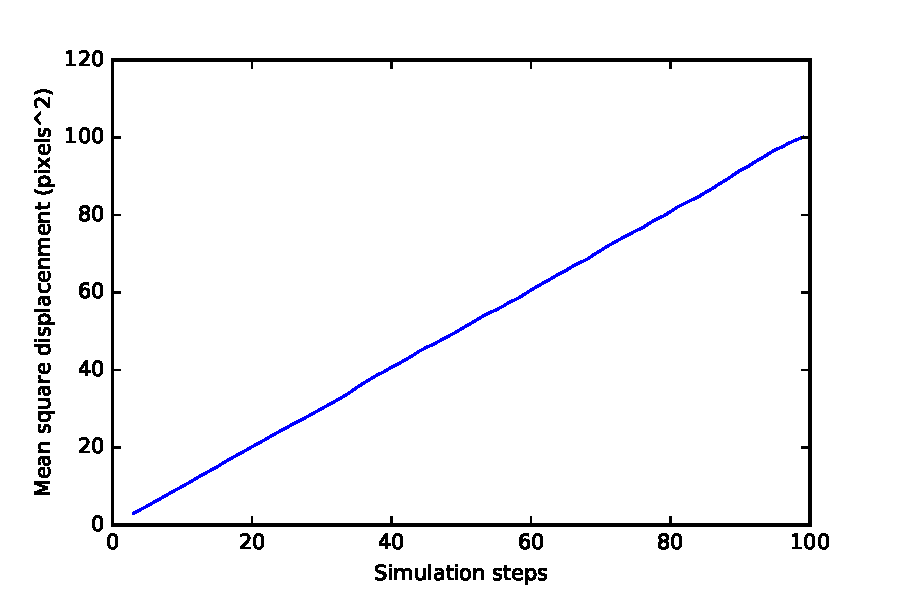
\includegraphics[width=.7\linewidth]{2Drandomwalk.pdf}
\caption{MSD vs time (simulation steps) for 10,000 random walks by a particle}
\label{fig:2Drandomwalk}
\end{figure}


\subsection*{b) Validation}

As seen in Figure \ref{fig:2Drandomwalk}, the mean square displacement \( <x>^2 \) scales linearly with time, as one would expect with diffusive movement. In this case, an 'eyeball' fit reveals the slope of the line appears to be \( \approx 1  \). To obtain the diffusion constant \( D \), we go through the following steps: 

\[ 4Dt = <x>^2 \]

\[ \rightarrow D = \frac{\Delta<x>^2}{4\Delta t} \approx 1 \]

\[ \rightarrow D \approx \frac{1}{4}  distance^2/time     \]

\section{Macroscopic Diffusion in 1-D}

\subsection*{a) Expected value}
We start from the definition of the expectation value, with Normal Distribution:
\begin{equation}\label{1}
  \rho(x,t)=\frac{1}{\sqrt{2\pi\sigma(t)^2}}exp(-\frac{x^2}{2\sigma(t)^2})
\end{equation}\\
the expectation value of $\langle x(t)^2 \rangle$ is defined as:
\begin{equation}\label{2}
  \langle x(t)^2 \rangle =\int_{-\infty}^{+\infty}x^2\rho(x,t)dx
\end{equation}\\
Then we solve the integral as follows using gamma function:
\begin{equation}\label{3}
  \begin{split}
  \langle x(t)^2 \rangle=&\frac{1}{\sqrt{2\pi\sigma(t)^2}}\int_{-\infty}^{+\infty}x^2exp(-\frac{x^2}{2\sigma(t)^2})dx\\
                        =&\frac{1}{\sqrt{2\pi\sigma(t)^2}}\times 2\int_{0}^{+\infty}(\frac{x}{\sqrt{2\sigma(t)^2}})^2
                           exp(-(\frac{x}{\sqrt{2\sigma(t)^2}})^2)d(\frac{x}{\sqrt{2\sigma(t)^2}})\times (2\sigma(t)^2)^{3/2}\\
                        =&\frac{2\sigma(t)^2}{\sqrt{\pi}}\times 2\int_{0}^{+\infty}t^2exp(-t^2)dt\\
                        =&\frac{2\sigma(t)^2}{\sqrt{\pi}}\Gamma(\frac{3}{2})\\
                        =&\frac{2\sigma(t)^2}{\sqrt{\pi}}\times \frac{1}{2}\sqrt{\pi}\\
                        =&\sigma(t)^2 \\
  \end{split}
\end{equation}\\


\subsection*{b) Numerical solution and validation}

Macroscopic diffusion in one dimension can be modeled using Fick's law:

\[ \frac{\partial u }{ \partial t} = D\frac{\partial ^2 u }{ \partial x^2}   \]

where \(u\) is the spatial concentration profile of a chemical at a give time, \(D\) is the diffusion constant, \(t\) is time, and \(x\) is distance. The discretized version is 
\( \frac{\Delta u }{ \Delta t} = D\frac{\Delta ^2 u }{ \Delta x^2}   \).

To solve this numerically, we utilize the following explicit method:

\[ c^{t+1}_{x} = k \times (c^{t}_{x+1} - 2 c^{t}_{x} + c^{t}_{x-1}    ) \]

The concentration of a cell at a future time step (\( c^{t+1}_{x} \)) is calculated using the concentration at the current time step ( \(c^{t}_{x}\) ) and the concentrations of adjacent cells ( \( c^{t}_{x+1}, c^{t}_{x-1} \)   ). Here,  \(k = D\frac{\Delta t}{\Delta x^2}\).

The evolving concentration profile of a box profile is shown in Figure \ref{fig:diffusiongraph} and a comparison between \(\sqrt[]{2Dt}\) and variance of normal fits is shown in Table \ref{table:1}.

\begin{figure}[H]
\centering
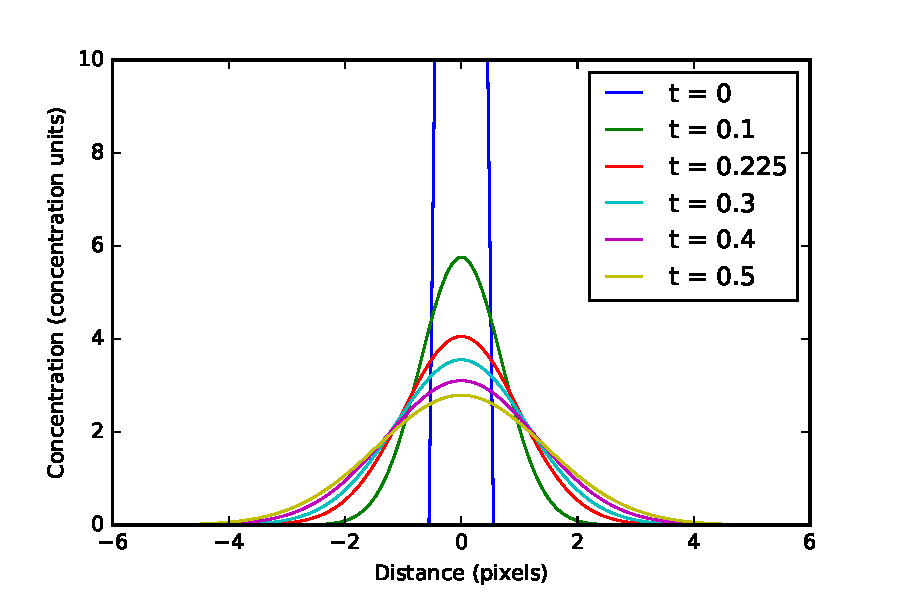
\includegraphics[width=.7\linewidth]{diffusiongraph.pdf}
\caption{Spatial concentration profile of a diffusing chemical. Different colors represent snapshots of the chemical's concentration profile taken at different times. }
\label{fig:diffusiongraph}
\end{figure}

\begin{tabular}{  c |  c | c }

\label{table:1}

\(\sqrt[]{2Dt}\) (in pixels) & Fit Value (in pixels) & Time (in time units)\\
\hline
0.63 & 0.69 & 0.1\\
0.94 & 0.99 & 0.225\\
1.10 & 1.13 & 0.3\\
1.26 & 1.29 & 0.4\\
1.41 & 1.43 & 0.5

\end{tabular}


\section{Diffusion-limited Aggregation}

\subsection*{Overview of DLA}
Diffusion-limited aggregation (DLA) is a process in which particles undergoing a random walk cluster together to form aggregates.  The clusters formed in DLA are fractals known as Brownian trees.   In two dimensions the fractals typically exhibit a dimension of around 1.65-1.71 for free particles that are unrestricted by a lattice, however, computer simulation of DLA requires cluster growth on a lattice structure which changes the fractal dimension slightly (so that it is closer to 1.5).  Another factor which alters the fractal dimension is the geometry of the growth, whether it be from a single point radially outward or from a plane or line.

\subsection*{a) Diffusion-limited aggregation (DLA) with periodic boundary conditions}

To simulate the DLA, a seed was placed at the origin, and random walkers were generated on a circle of radius = 100 distance units. Periodic boundary conditions were used to ensure the particle would not wander away from the cluster (hence, the particle didn't need to have a lifetime). Once the cluster grew to a certain size ( \(\approx 100\) distance units in radius ), the simulation was terminated.



\subsection*{b) and c)  Extraction of Fractal Dimension }
The fractal dimension of the cluster can be extracted by plotting the "mass"  (number of  pieces of the cluster) as a function of radius. This was performed ten times, and the average fractal dimension for each run was extracted and found to be 1.517 , consistent with the theoretical value for general DLA on a  lattice structure.   The resultant cluster and plots for the mass as a function of radius are shown for 3 representative samples.  


\begin{figure}[H]
\centering
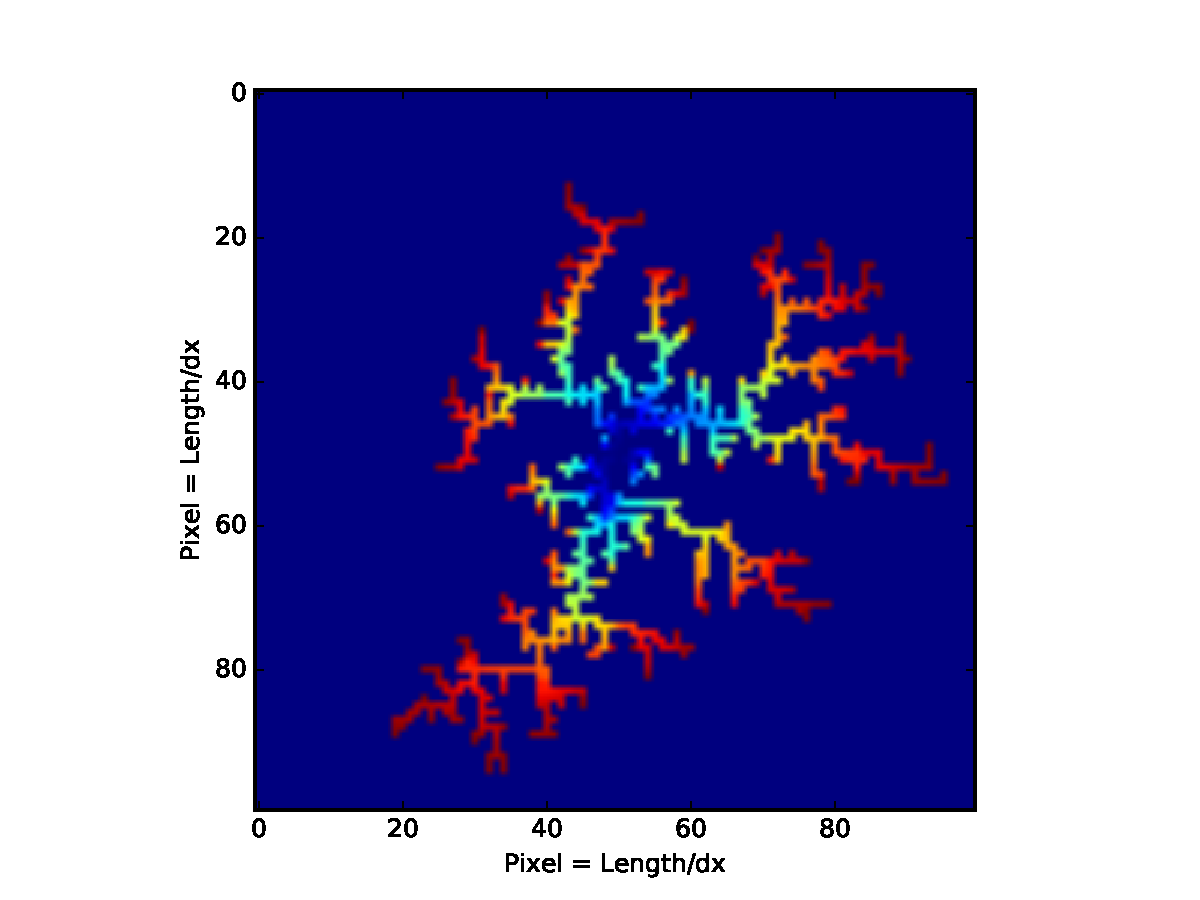
\includegraphics[width=.9\linewidth]{Cluster1.pdf}
\caption{Sample cluster formed via DLA. Length = 200, dx = 2}
\label{fig:Cluster1}
\end{figure}

\begin{figure}[H]
\centering
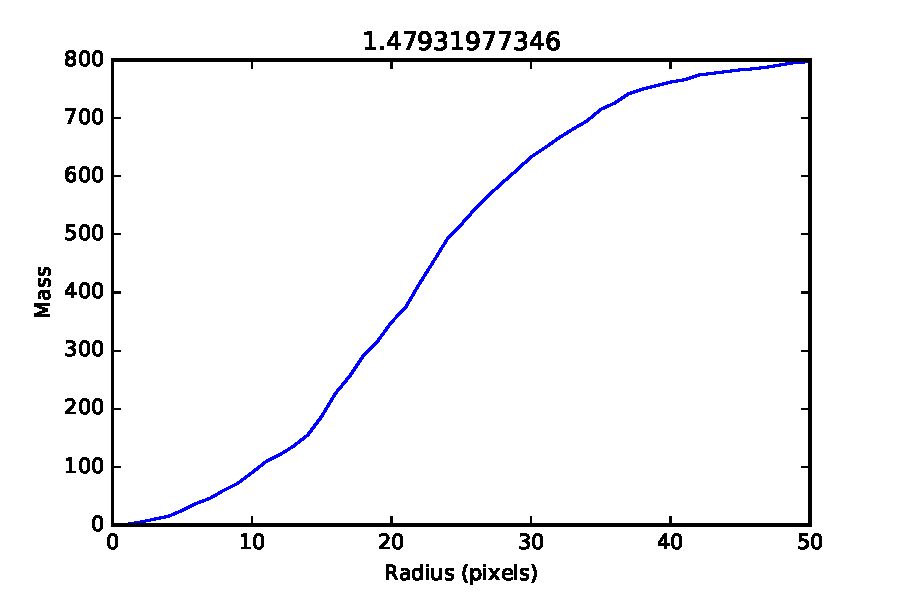
\includegraphics[width=.9\linewidth]{Cluster1dim.pdf}
\caption{Mass as a function of radius for cluster 1}
\label{fig:Fractal Dimension Plot for Cluster 1}
\end{figure}

\begin{figure}[H]
\centering
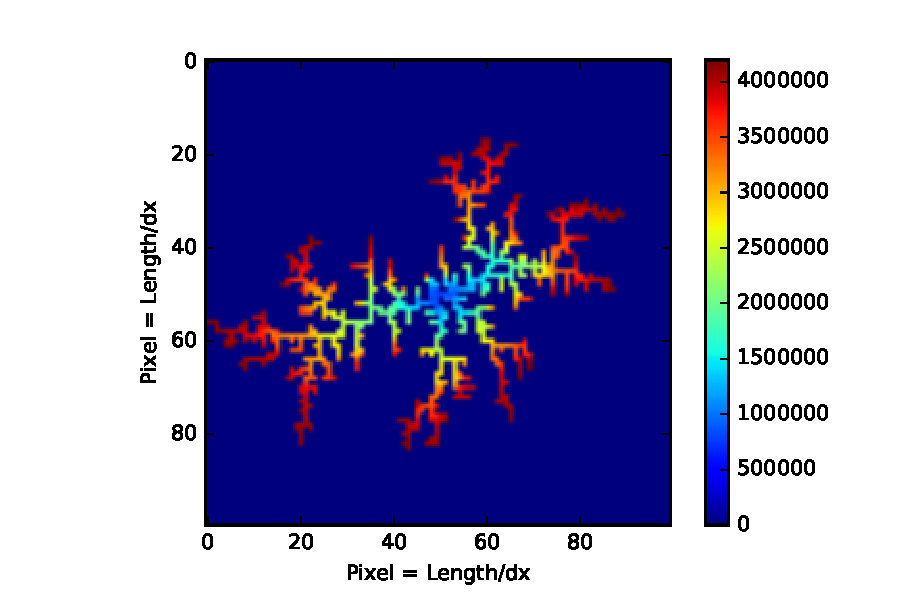
\includegraphics[width=.9\linewidth]{Cluster2.pdf}
\caption{Sample cluster formed via DLA. Length = 200, dx = 2}
\label{fig:Cluster2}
\end{figure}

\begin{figure}[H]
\centering
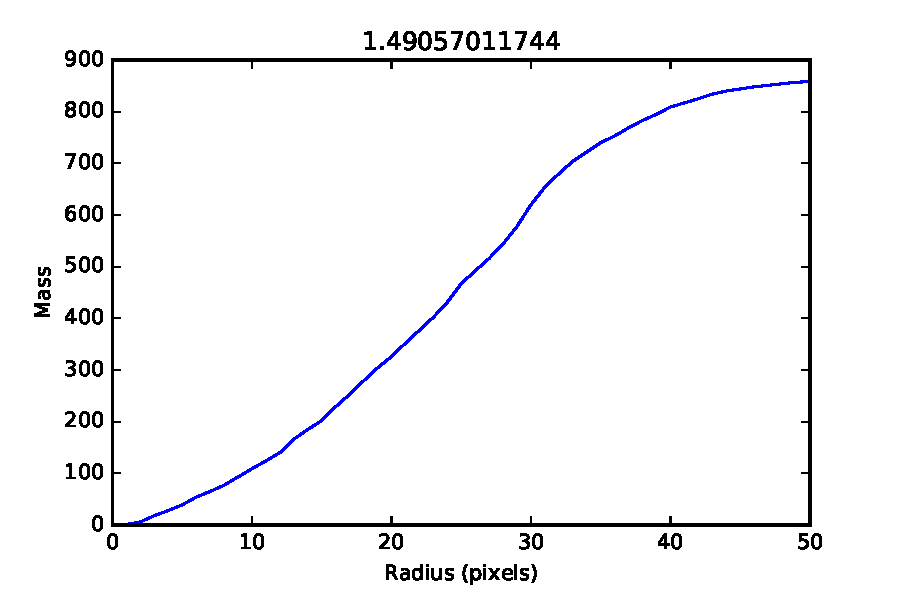
\includegraphics[width=.9\linewidth]{Cluster2dim.pdf}
\caption{Mass as a function of radius for cluster 2}
\label{fig:Fractal Dimension Plot for Cluster 2}
\end{figure}


\begin{figure}[H]
\centering
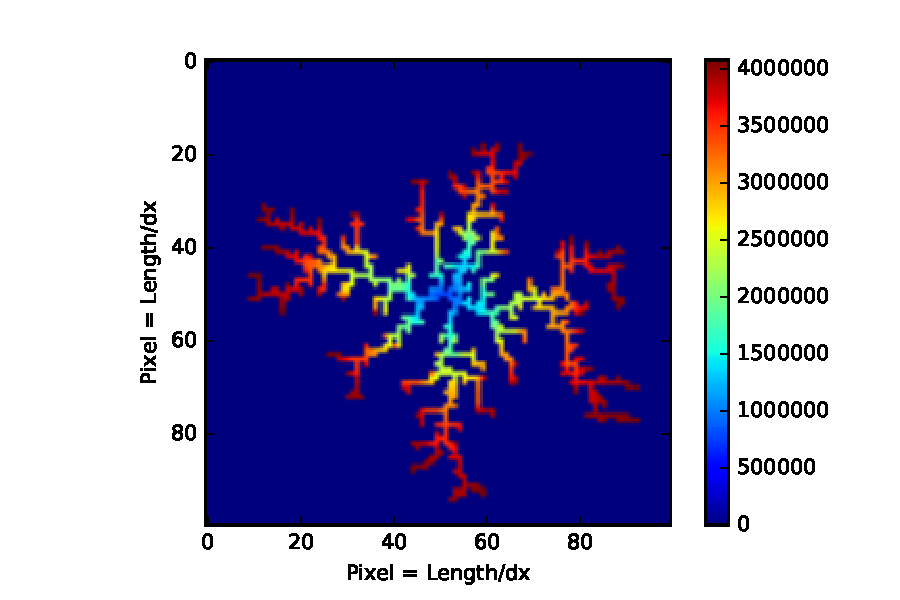
\includegraphics[width=.9\linewidth]{Cluster3.pdf}
\caption{Sample cluster formed via DLA. Length = 200, dx = 2}
\label{fig:Cluster3}
\end{figure}





\end{document}